\iffalse
\documentclass{article}
% Language setting
% Replace `english' with e.g. `spanish' to change the document language
\usepackage[english]{babel}
% Set page size and margins
% Replace `letterpaper' with `a4paper' for UK/EU standard size
\usepackage[letterpaper,top=2cm,bottom=2cm,left=3cm,right=3cm,marginparwidth=1.75cm]{geometry}
% Useful packages
\usepackage{multicol}
\usepackage{amsmath}
\usepackage{amssymb}
\usepackage{graphicx}
\usepackage[framemethod=tikz]{mdframed}
\usepackage{array}
\usepackage{blindtext}
%\usepackage[paperwidth=10cm]{geometry}
\usepackage{tkz-euclide}
%\usepackage{tikz}
\usetikzlibrary{
  circuits.logic,
  circuits.logic.US,
  positioning
}

\usepackage[colorlinks=true, allcolors=blue]{hyperref}
\newcommand{\myvec}[1]{\ensuremath{\begin{pmatrix}#1\end{pmatrix}}}
\providecommand{\norm}[1]{\left\lVert#1\right\rVert}
\let\vec\mathbf
\title{Optimization Assignment-1}
\author{Ballepu dheeraj kumar}
\begin{document}
\maketitle
\newtheorem{theorem}{Theorem}[section]
\begin{multicols}{2}

\paragraph{\begin{flushleft}\textbf{Problem: }
\fi
Minimise and Maximise
\begin{align}
Z = 5x+10y
\end{align}
subject to
\begin{align}
	x+2y &\le 120
	\\
	x+y &\ge 60
	\\
	x-2y &\ge 0
	\\
	x \ge 0 , y &\ge 0
\end{align}
\solution
	\begin{figure}[!ht]
		\centering
		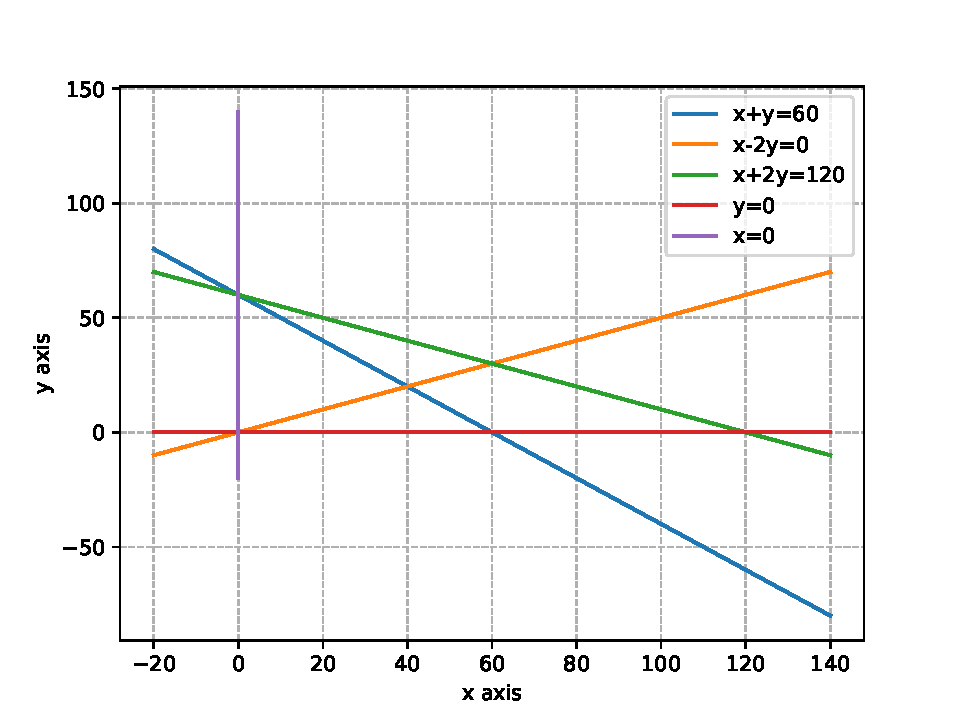
\includegraphics[width=\columnwidth]{12/12/1/7/figs/opt1.pdf}
		\caption{}
		\label{fig:12/12/1/7}
  	\end{figure}
	\iffalse
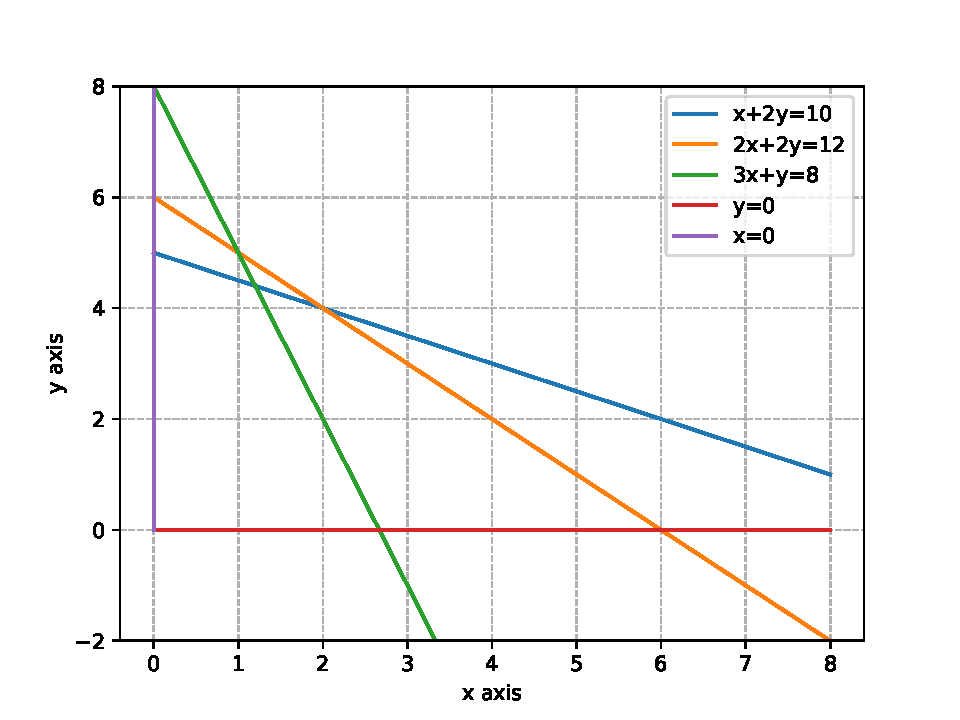
\includegraphics[scale=0.5]{/sdcard/Download/Opti/figure2/opt1.pdf} 
\end{flushleft}}
\section*{Solution}
\begin{flushleft}
\begin{align}
\min_{\vec{x}} Z=(5x+10y)\\
\max_{\vec{x}} Z=(5x+10y) \\
\end{align}
\begin{align*}
x+2y \preceq 120
\end{align*}
\begin{align*}
x+y \succeq 60
\end{align*}
\begin{align*}
x-2y \succeq 60
\end{align*}
\begin{align*}
x \succeq 0 , y \succeq 0
\end{align*}
all the above expressions can be expressed in vector form as
\fi
	The given 
problem can be formulated as
\begin{align}
	\min_{\vec{x}}\vec{Z}=\myvec{5 & 10}\vec{x}\\
	\max_{\vec{x}}\vec{Z}=\myvec{5 &10}\vec{x}\\
	s.t. \quad
	\myvec{
	-1 & -2 \\
		1 &1\\
	1 & -2\\
	1 &0\\
	0 &1
	}\vec{x}\succeq \myvec{-120 \\ 60 \\0\\0\\0}\\   
\end{align}
%\begin{align}
%\max_{\vec{x}}\vec{Z}=\myvec{5 \hspace{0.2cm}10}\vec{x}\\
%\myvec{1 \hspace{0.2cm}2\vec{x}\preceq \myvec{120}
%\end{align}
Solving above equations using cvxpy,
\begin{align}
\min_{\vec{x}} Z=300,
\vec{x}=\myvec{60\\0}
\\
\max_{\vec{x}} Z=600,
\vec{x}=\myvec{60\\30}
\end{align}
\iffalse
\end{multicols}{2}
\end{document}
\fi
